\documentclass[paper=A4, fontsize=11pt, titlepage]{article}

\usepackage[utf8]{inputenc}
\usepackage[T1]{fontenc} 
\usepackage{fourier} 
\usepackage[english]{babel}
\usepackage{graphicx}
\usepackage{amsmath,amsfonts,amsthm} 
\usepackage{fancyhdr} 
\usepackage{titlesec}
\usepackage[super]{nth}

\pagestyle{fancy}
\renewcommand{\sectionmark}[1]{ \markboth{#1}{} }
\setlength{\headheight}{24pt}
\fancyhf[HL]{\raisebox{-0.4\height}{
\includegraphics[height=24pt]{fig/udemheader}}}
\fancyhead[HC]{\leftmark}
\fancyhf[HR]{\raisebox{-0.4\height}{
\includegraphics[height=24pt]{fig/esisarheader}}}
\fancyhf[FC]{\thepage}

\titleformat{\section}
{\normalfont\Large\bfseries}{\thesection}{1em}{}
[\normalfont\small\itshape\raggedleft\sectionpostamble\global\let\sectionpostamble\relax]

\numberwithin{equation}{section}
\numberwithin{figure}{section}
\numberwithin{table}{section}

\setlength\parindent{0pt}

\newcommand{\horrule}[1]{\rule{\linewidth}{#1}} 
\newcommand*{\sectionpostamble}{}
\newcommand*{\fromto}[1]{\def\sectionpostamble{#1}}

%%%%%%%%%%%%%%%%%%%%%%%%%%%%%%%%%%%%%%%%%%%%%%%
\begin{document}

  \begin{titlepage}
%    \vspace*{\fill}
    \begin{center}
	
\includegraphics[height=0.35\textwidth]{fig/udemlogo}\\
	\vspace{2mm}
	\huge UNIVERSIDAD DE MONTERREY\\
	\vspace{1mm}
	\Large División de Ingeniería y Tecnologías\\
	\vspace{1mm}
	\large Departamento de Inegniería\\
	\vspace{10mm}
	\horrule{1pt} \\[0.4cm]
	\Huge ACTIVITIES REPORT\\ 
	\large Final Evaluation Project\\
	\horrule{2pt} \\[0.5cm]
	\vspace{10mm}
	\Large\raggedright Dr. Jorge de Jesús Lozoya Santos\\
	\normalsize\raggedright Project Assessor\\
	\vspace{10mm}
	\Large\raggedleft Pedro Aguiar\\
	\normalsize\raggedleft Mechatronics Engineering Student\\
	\vspace{20mm}
	\Large\centering May \nth{16}, 2014.\\
    \end{center}
%    \vspace*{\fill}
  \end{titlepage}

\tableofcontents
\clearpage
\listoffigures
\listoftables
\clearpage

%%%%%%%%%%%%%%%%%%%%%%%%%%%%%%%%%%%%%%%%%%%%%%%

\fromto{April 23 - Mayo 2}
\section{MEMORANDUM 01}

\subsection{Proceso Administrativo}
En esta semana todavía hubo pendientes administrativos que se reportan a continuación, como referencia e información para futuros estudiantes de la UDEM que vayan a participar en un programa similar. Al llegar al laboratorio lo primero que hiceron fue llevarme con Jennyfer DUBERVILLE para revisar los procedimientos administrativos. Se revisó que la papelería que había sido enviada por internet estuviera correcta. La papelería consistió en:
\begin{itemize}
	\item Credencial de estudiante
	\item Copia del último certificado (en mi caso el de la preparatoria)
	\item Copia del pasaporte
	\item Un contrato (firmado por mí y por el director de DIT, por parte de la UDEM)
\end{itemize}
Después de corroborar la papelería se le entregó un formulario a mi asesor y a mí me dieron un reglamento acerca del uso de los recursos del laboratorio (internet, equipo electrónico, etcétera). Se me hizo firmar un papel en el que decía la fecha de llegada al laboratorio y donde declaraba haber leído el reglamento. Se me recordó que los primeros días de Mayo tendría que pagar las cuotas de "social security" y "civil liability". También se me informó que pare recibir la gratificación tengo que abrir una cuenta en un banco Francés y me dijeron que me iban a contactar con una persona que podía ayudarme con eso.

Por último se me proporcionaron las credenciales de acceso a Internet y mi computadora. Se instaló el equipo de cómputo que se me asignó y se me explicó cómo utilizarlo, así como algunos comentarios finales (no se puede conectar nada a la red alámbrica, no puedo instalar software que no esté en los repositorios de Debian, cómo acceder a mi espacio en el servidor de la escuela que está respaldado, detalles de ese tipo).


\subsection{Actividades}

\subsubsection{PCB comunicación entre cámara y raspberry pi.}
Durante el primer día de trabajo se hizo un bill of materials (Tabla \ref{tab_bompic}) para hacer una tarjeta de circuito impreso que conecte una cámara OV7670 con el raspberry, el objetivo siendo que el Carrita tenga capacidades de visión computarizada. La diferencia con la de la UDEM es que Varrier externó que le gustaría recibir en el raspberry:
\begin{itemize}
	\item Máxima resolución (640x480).
	\item Máximo framerate (30fps).
	\item Imagen a color.
\end{itemize}
\begin{table}
\begin{center}
\begin{tabular}{| l | c | c | c |}
\hline
\multicolumn{1}{|c|}{Componente}	 & 	\multicolumn{1}{c|}{Cant.}	 & 	\multicolumn{1}{c|}{Precio Unitario} & 	\multicolumn{1}{c|}{Costo (euros)}\\ \hline
PIC18F45K80-I/P	 & 	1	 & 	3.46	 & 	3.46\\ \hline
Capacitor cerámico 0.1 uF	 & 	10	 & 	0.386	 & 	3.86\\ \hline
Capacitor cerámico 1 nF	 & 	25	 & 	0.114	 & 	2.85\\ \hline
Capacitor tantalum 10 uF	 & 	5	 & 	0.822	 & 	4.11\\ \hline
Capacitor cerámico 15 pF	 & 	10	 & 	0.262	 & 	2.62\\ \hline
Resistor 470 ohm	 & 	10	 & 	0.034	 & 	0.34\\ \hline
Resistor 10k	 & 	10	 & 	0.025	 & 	0.25\\ \hline
Resistor 330	 & 	10	 & 	0.034	 & 	0.34\\ \hline
Resistor 470	 & 	10	 & 	0.034	 & 	0.34\\ \hline
Cable (jumper terminals)	 & 	30	 & 	0	 & 	0\\ \hline
Headers (pins)	 & 	2	 & 	3.43	 & 	6.86\\ \hline
Quartz	 & 	1	 & 	2.11	 & 	2.11\\ \hline
Switch SPDT	 & 	3	 & 	2.27	 & 	6.81\\ \hline
PicKit2	 & 	1	 & 	33.99	 & 	33.99\\ \hline
\multicolumn{2}{c|}{}	 & 	Subtotal	 & 	67.94\\ \cline{3-4}
\multicolumn{2}{c|}{}	& 	Total	 & 	81.528\\ \cline{3-4}
  \end{tabular}
\caption{Bill of materials para el PCB de conexión entre el PIC y la cámara.}
\label{tab_bompic}
\end{center}
\end{table}

Observaciones sobre el bill of materials:
\begin{itemize}
	\item Costo elevado
	\begin{itemize}
		\item 40.74 euros de componentes de una placa.
		\item 33.99 euros para el programador.
	\end{itemize}
	\item El proveedor impone cantidades mínimas de componentes.
	\item No está considerado el costo de mandar a hacer la placa.
	\item No se podría utilizar el microcontrolador de la UDEM porque no estaban considerados los bits para el color.
	\item Por lo tanto, el PCB tendría que ser diseñado completamente desde cero con la sensación (personal) de menos herramientas y proveedores menos accesibles.
\end{itemize}

%%%%%%%%%%%%%%%%%%%%%%%%%%%%%%%%%%%%%%%%%%%%%%%%%%%%%%%%%%%%%%%%%%%%%%%

\subsubsection{Alternativa a Microchip.}
Debido a lo costoso en dinero (componentes) y tiempo (diseño y armado) que resultó ser el diseño de un PCB para establecer la comunicación con las cámaras procedí a buscar una alternativa que ofrecerle a Varrier. La mejor alternativa fue utilizar un STM32, porque:
\begin{itemize}
	\item Tienen Digital Camera Module Interface (DCMI).
	\item Tienen Direct Memory Access (DMA).
	\item Combinando DCMI+DMA se pueden guardar frames en memoria usando sólo hardware (el procesador queda libre para usarlo para otras aplicaciones).
	\item Hay tarjetas de evaluación de bajo costo (una de 12 y otra de 21 euros).
	\item Programación por USB.
	\item Varrier tiene experiencia y confianza en estos dispositivos.
\end{itemize}

Se investigó para validar que las tarjetas de evaluación pudieran hacer la comunicación con la cámara. También se revisó si se podrían utilizar los sensores y la pantalla LCD de la tarjeta (si no interferían con los pines que se necesitaban para la cámara). Se tomó la decisión de comprar dos tarjetas 32F429IDISCOVERY.

%%%%%%%%%%%%%%%%%%%%%%%%%%%%%%%%%%%%%%%%%%%%%%%%%%%%%%%%%%%%%%%%%%%%%%%

\subsubsection{Estudio e implementación en C de transformada de Hough.}
El código implementado en la UDEM para detectar la línea que se está siguiendo utiliza OpenCV, una librería que tiene una gran variedad de algoritmos para hacer visión computarizada. Es un objetivo del proyecto que el Carrita pueda medir la distancia que hay hacia un vehículo que esté enfrente y esta función no estaba implementada.

Antes de comenzar la implementación decidí deshacerme de la dependencia de OpenCV y desarrollar código en C para una transformada de Hough basado en los siguientes hechos:

\begin{itemize}
	\item OpenCV es una librería muy generalizada con una gran cantidad de funciones (la descarga de la versión estable actual, 2.4.9 es de más de 87MB para Linux).
	\item Para la detección de línea sólo se estaban usando dos "funciones complejas" de OpenCV.
	\begin{itemize}
		\item Canny edge detector.
		\item Hough transform.
		\item Seguramente menos del 0.5\% de los 87MB.
	\end{itemize}
	\item La transformada de Hough de OpenCV no puede usarse para detectar al vehículo de enfrente (sólo se detectan líneas rectas y círculos).
	\item OpenCV hace el cálculo completo de la transformada en cada frame. Nuestra aplicación puede aprovechar el hecho de saber que es un video para no realizar el cálculo completo en cada frame y buscar alrededor del punto conocido del cálculo anterior.
\end{itemize}

Además tenemos las ventajas típicas de programar una versión independiente de librerías:
\begin{itemize}
	\item Conocimiento profundo de la transformada (funcionalidad menos abstracta).
	\item Adaptación específica a la necesidad (minimalista, rápida, a la medida).
	\item Libertad en funcionalidad, optimizaciones e interfaces.
\end{itemize}

En algún momento se iba a llegar al límite de la capacidad del raspberry utilizando OpenCV y para empujar ese límite se tendría que bajar a una solución específica sin uso de librerías generalizadas.

Para implementar en C la transformada de Hough se llevaron a cabo las siguientes tareas:

\begin{itemize}
	\item Estudio de la teoría detrás de la transformada de Hough.
	\item Búsqueda y comparación de código existente para la transformada.
	\item Adaptar una versión a usar sólo C (sustituir librerías).
	\item Implementar optimizaciones
	\begin{itemize}
		\item (Ab)uso del preprocesador (para reducir bifurcaciones). 
		\item Aritmética de punto fijo.
		\item Tablas de funciones trigonométricas.
		\item Memoria asignada estáticamente.
		\item Region de interés.
		\item Reducción de grados de libertad.
	\end{itemize}
\end{itemize}

Se utilizó SDL para dibujar en pantalla (no es necesario, pero sirve para ver y comprobar resultados) y se adaptó fast-edge (http://goo.gl/ARWJZj), un proyecto encontrado en internet, para hacer detección de bordes.

%%%%%%%%%%%%%%%%%%%%%%%%%%%%%%%%%%%%%%%%%%%%%%%%%%%%%%%%%%%%%%%%%%%%

\subsubsection[Revisión bibliográfica transformada de Hough.]{Revisión bibliográfica de aplicaciones de la transformada de Hough.}
Se han descargado 25 artículos relevantes al tema en los que se están observando aplicaciones de extracción de características usando la transformada de Hough. Al seleccionarlos se observó que hablan de las limitantes de la transformada, pequeñas modificaciones para resolverlas, así como propuestas y resultados experimentales.



\subsection{Resultados}

\subsubsection{PCB comunicación entre cámara y raspberry pi}
\begin{itemize}
	\item Bill of materials de la tabla \ref{tab_bompic}.
	\item Debido al costo elevado en tiempo y dinero se decidió buscar una alternativa.
\end{itemize}

\subsection{Alternativa a Microchip}
\begin{itemize}
	\item Se utilizará un STM32.
	\item La tarjeta a utilizar es la 32F429IDISCOVERY.
\end{itemize}

\subsection{Estudio e implementación en C de transformada de Hough}
\begin{itemize}
	\item Se entendió toda la teoría detrás de la transformada.
	\item Se implementó la funcionalidad de la transformada de Hough tradicional utilizando sólo C.
\end{itemize}

\subsubsection{Revisión bibliográfica de aplicaciones de la transformada de Hough.}
\begin{itemize}
	\item Empecé una revisión bibliográfica
	\item Observé las modificaciones (y su justificación) que se hacen a la transformada de Hough "tradicional" para implementarla en aplicaciones reales.
\end{itemize}


\subsection{Pendientes}

\begin{itemize}
\item \textbf{Gantt:} Le puedo adelantar que Varrier y yo estuvimos de acuerdo en que en dos meses tenemos que haber hecho el control de distancia (y de ser posible también lateral) utilizando las cámaras y haber envíado un artículo a alguna conferencia. Después de esos dos meses me dijo que lo decidiriamos después en base a mis intereses, etcétera. La única opción que le ofrecí fue la de simular la flotilla de vehículos y le pareció buena idea pero me dijo que lo siguiera pensando y cuando estuviera la fecha más cercana tomábamos la decisión. Entiendo algo como que el plan de colaborar con otro equipo (que se iba a encargar de la simulación de la flotilla) se vino abajo.
\item \textbf{Compras:} La próxima semana estarán llegando los componentes.
\item \textbf{Repositorio y Dropbox:} Estuve buscando una forma de sincronizar y respaldar el trabajo, ya me rendí y parece que no habrá formas cómodas (por restricciones de no instalar software que no esté en los repositorios de Debian y debido a que estamos atrás de un proxy que necesita contraseñas), pero aun así subiré todo el trabajo a algún lugar, le aviso la decisión en el próximo reporte.
\item \textbf{Las actividades se dibujan así:} programación de STM32, trabajo electrónico para envíar las imágenes de la cámara al raspberry, desarrollo de transformada de hough específica para la aplicación, sacar modelos adecuados para la aplicación, implementar control tolerante a fallas.
\end{itemize}

\clearpage

%%%%%%%%%%%%%%%%%%%%%%%%%%%%%%%%%%%%%%%%%%%%%%%

\fromto{May 5 - May 9}
\section{MEMORANDUM 02}

\subsection{Actividades}

\subsubsection{PCB comunicación entre cámara y raspberry pi.}
Durante el primer día de trabajo se hizo un bill of materials (Tabla \ref{tab_bompic}) para hacer una tarjeta de circuito impreso que conecte una cámara OV7670 con el raspberry, el objetivo siendo que el Carrita tenga capacidades de visión computarizada. La diferencia con la de la UDEM es que Varrier externó que le gustaría recibir en el raspberry:
\begin{itemize}
	\item Máxima resolución (640x480).
	\item Máximo framerate (30fps).
	\item Imagen a color.
\end{itemize}
\begin{table}
\begin{center}
\begin{tabular}{| l | c | c | c |}
\hline
\multicolumn{1}{|c|}{Componente}	 & 	\multicolumn{1}{c|}{Cant.}	 & 	\multicolumn{1}{c|}{Precio Unitario} & 	\multicolumn{1}{c|}{Costo (euros)}\\ \hline
PIC18F45K80-I/P	 & 	1	 & 	3.46	 & 	3.46\\ \hline
Capacitor cerámico 0.1 uF	 & 	10	 & 	0.386	 & 	3.86\\ \hline
Capacitor cerámico 1 nF	 & 	25	 & 	0.114	 & 	2.85\\ \hline
Capacitor tantalum 10 uF	 & 	5	 & 	0.822	 & 	4.11\\ \hline
Capacitor cerámico 15 pF	 & 	10	 & 	0.262	 & 	2.62\\ \hline
Resistor 470 ohm	 & 	10	 & 	0.034	 & 	0.34\\ \hline
Resistor 10k	 & 	10	 & 	0.025	 & 	0.25\\ \hline
Resistor 330	 & 	10	 & 	0.034	 & 	0.34\\ \hline
Resistor 470	 & 	10	 & 	0.034	 & 	0.34\\ \hline
Cable (jumper terminals)	 & 	30	 & 	0	 & 	0\\ \hline
Headers (pins)	 & 	2	 & 	3.43	 & 	6.86\\ \hline
Quartz	 & 	1	 & 	2.11	 & 	2.11\\ \hline
Switch SPDT	 & 	3	 & 	2.27	 & 	6.81\\ \hline
PicKit2	 & 	1	 & 	33.99	 & 	33.99\\ \hline
\multicolumn{2}{c|}{}	 & 	Subtotal	 & 	67.94\\ \cline{3-4}
\multicolumn{2}{c|}{}	& 	Total	 & 	81.528\\ \cline{3-4}
  \end{tabular}
\caption{Bill of materials para el PCB de conexión entre el PIC y la cámara.}
\label{tab_bompic}
\end{center}
\end{table}

Observaciones sobre el bill of materials:
\begin{itemize}
	\item Costo elevado
	\begin{itemize}
		\item 40.74 euros de componentes de una placa.
		\item 33.99 euros para el programador.
	\end{itemize}
	\item El proveedor impone cantidades mínimas de componentes.
	\item No está considerado el costo de mandar a hacer la placa.
	\item No se podría utilizar el microcontrolador de la UDEM porque no estaban considerados los bits para el color.
	\item Por lo tanto, el PCB tendría que ser diseñado completamente desde cero con la sensación (personal) de menos herramientas y proveedores menos accesibles.
\end{itemize}

%%%%%%%%%%%%%%%%%%%%%%%%%%%%%%%%%%%%%%%%%%%%%%%%%%%%%%%%%%%%%%%%%%%%%%%

\subsubsection{Alternativa a Microchip.}
Debido a lo costoso en dinero (componentes) y tiempo (diseño y armado) que resultó ser el diseño de un PCB para establecer la comunicación con las cámaras procedí a buscar una alternativa que ofrecerle a Varrier. La mejor alternativa fue utilizar un STM32, porque:
\begin{itemize}
	\item Tienen Digital Camera Module Interface (DCMI).
	\item Tienen Direct Memory Access (DMA).
	\item Combinando DCMI+DMA se pueden guardar frames en memoria usando sólo hardware (el procesador queda libre para usarlo para otras aplicaciones).
	\item Hay tarjetas de evaluación de bajo costo (una de 12 y otra de 21 euros).
	\item Programación por USB.
	\item Varrier tiene experiencia y confianza en estos dispositivos.
\end{itemize}

Se investigó para validar que las tarjetas de evaluación pudieran hacer la comunicación con la cámara. También se revisó si se podrían utilizar los sensores y la pantalla LCD de la tarjeta (si no interferían con los pines que se necesitaban para la cámara). Se tomó la decisión de comprar dos tarjetas 32F429IDISCOVERY.

%%%%%%%%%%%%%%%%%%%%%%%%%%%%%%%%%%%%%%%%%%%%%%%%%%%%%%%%%%%%%%%%%%%%%%%

\subsubsection{Estudio e implementación en C de transformada de Hough.}
El código implementado en la UDEM para detectar la línea que se está siguiendo utiliza OpenCV, una librería que tiene una gran variedad de algoritmos para hacer visión computarizada. Es un objetivo del proyecto que el Carrita pueda medir la distancia que hay hacia un vehículo que esté enfrente y esta función no estaba implementada.

Antes de comenzar la implementación decidí deshacerme de la dependencia de OpenCV y desarrollar código en C para una transformada de Hough basado en los siguientes hechos:

\begin{itemize}
	\item OpenCV es una librería muy generalizada con una gran cantidad de funciones (la descarga de la versión estable actual, 2.4.9 es de más de 87MB para Linux).
	\item Para la detección de línea sólo se estaban usando dos "funciones complejas" de OpenCV.
	\begin{itemize}
		\item Canny edge detector.
		\item Hough transform.
		\item Seguramente menos del 0.5\% de los 87MB.
	\end{itemize}
	\item La transformada de Hough de OpenCV no puede usarse para detectar al vehículo de enfrente (sólo se detectan líneas rectas y círculos).
	\item OpenCV hace el cálculo completo de la transformada en cada frame. Nuestra aplicación puede aprovechar el hecho de saber que es un video para no realizar el cálculo completo en cada frame y buscar alrededor del punto conocido del cálculo anterior.
\end{itemize}

Además tenemos las ventajas típicas de programar una versión independiente de librerías:
\begin{itemize}
	\item Conocimiento profundo de la transformada (funcionalidad menos abstracta).
	\item Adaptación específica a la necesidad (minimalista, rápida, a la medida).
	\item Libertad en funcionalidad, optimizaciones e interfaces.
\end{itemize}

En algún momento se iba a llegar al límite de la capacidad del raspberry utilizando OpenCV y para empujar ese límite se tendría que bajar a una solución específica sin uso de librerías generalizadas.

Para implementar en C la transformada de Hough se llevaron a cabo las siguientes tareas:

\begin{itemize}
	\item Estudio de la teoría detrás de la transformada de Hough.
	\item Búsqueda y comparación de código existente para la transformada.
	\item Adaptar una versión a usar sólo C (sustituir librerías).
	\item Implementar optimizaciones
	\begin{itemize}
		\item (Ab)uso del preprocesador (para reducir bifurcaciones). 
		\item Aritmética de punto fijo.
		\item Tablas de funciones trigonométricas.
		\item Memoria asignada estáticamente.
		\item Region de interés.
		\item Reducción de grados de libertad.
	\end{itemize}
\end{itemize}

Se utilizó SDL para dibujar en pantalla (no es necesario, pero sirve para ver y comprobar resultados) y se adaptó fast-edge (http://goo.gl/ARWJZj), un proyecto encontrado en internet, para hacer detección de bordes.

%%%%%%%%%%%%%%%%%%%%%%%%%%%%%%%%%%%%%%%%%%%%%%%%%%%%%%%%%%%%%%%%%%%%

\subsubsection[Revisión bibliográfica transformada de Hough.]{Revisión bibliográfica de aplicaciones de la transformada de Hough.}
Se han descargado 25 artículos relevantes al tema en los que se están observando aplicaciones de extracción de características usando la transformada de Hough. Al seleccionarlos se observó que hablan de las limitantes de la transformada, pequeñas modificaciones para resolverlas, así como propuestas y resultados experimentales.



\subsection{Resultados}

\subsubsection{PCB comunicación entre cámara y raspberry pi}
\begin{itemize}
	\item Bill of materials de la tabla \ref{tab_bompic}.
	\item Debido al costo elevado en tiempo y dinero se decidió buscar una alternativa.
\end{itemize}

\subsection{Alternativa a Microchip}
\begin{itemize}
	\item Se utilizará un STM32.
	\item La tarjeta a utilizar es la 32F429IDISCOVERY.
\end{itemize}

\subsection{Estudio e implementación en C de transformada de Hough}
\begin{itemize}
	\item Se entendió toda la teoría detrás de la transformada.
	\item Se implementó la funcionalidad de la transformada de Hough tradicional utilizando sólo C.
\end{itemize}

\subsubsection{Revisión bibliográfica de aplicaciones de la transformada de Hough.}
\begin{itemize}
	\item Empecé una revisión bibliográfica
	\item Observé las modificaciones (y su justificación) que se hacen a la transformada de Hough "tradicional" para implementarla en aplicaciones reales.
\end{itemize}


\subsection{Pendientes}

\begin{itemize}
\item \textbf{Gantt:} Le puedo adelantar que Varrier y yo estuvimos de acuerdo en que en dos meses tenemos que haber hecho el control de distancia (y de ser posible también lateral) utilizando las cámaras y haber envíado un artículo a alguna conferencia. Después de esos dos meses me dijo que lo decidiriamos después en base a mis intereses, etcétera. La única opción que le ofrecí fue la de simular la flotilla de vehículos y le pareció buena idea pero me dijo que lo siguiera pensando y cuando estuviera la fecha más cercana tomábamos la decisión. Entiendo algo como que el plan de colaborar con otro equipo (que se iba a encargar de la simulación de la flotilla) se vino abajo.
\item \textbf{Compras:} La próxima semana estarán llegando los componentes.
\item \textbf{Repositorio y Dropbox:} Estuve buscando una forma de sincronizar y respaldar el trabajo, ya me rendí y parece que no habrá formas cómodas (por restricciones de no instalar software que no esté en los repositorios de Debian y debido a que estamos atrás de un proxy que necesita contraseñas), pero aun así subiré todo el trabajo a algún lugar, le aviso la decisión en el próximo reporte.
\item \textbf{Las actividades se dibujan así:} programación de STM32, trabajo electrónico para envíar las imágenes de la cámara al raspberry, desarrollo de transformada de hough específica para la aplicación, sacar modelos adecuados para la aplicación, implementar control tolerante a fallas.
\end{itemize}

\clearpage

%%%%%%%%%%%%%%%%%%%%%%%%%%%%%%%%%%%%%%%%%%%%%%%

\fromto{May 12 - May 16}
\section{MEMORANDUM 03}

\subsection{Actividades}

\subsubsection{PCB comunicación entre cámara y raspberry pi.}
Durante el primer día de trabajo se hizo un bill of materials (Tabla \ref{tab_bompic}) para hacer una tarjeta de circuito impreso que conecte una cámara OV7670 con el raspberry, el objetivo siendo que el Carrita tenga capacidades de visión computarizada. La diferencia con la de la UDEM es que Varrier externó que le gustaría recibir en el raspberry:
\begin{itemize}
	\item Máxima resolución (640x480).
	\item Máximo framerate (30fps).
	\item Imagen a color.
\end{itemize}
\begin{table}
\begin{center}
\begin{tabular}{| l | c | c | c |}
\hline
\multicolumn{1}{|c|}{Componente}	 & 	\multicolumn{1}{c|}{Cant.}	 & 	\multicolumn{1}{c|}{Precio Unitario} & 	\multicolumn{1}{c|}{Costo (euros)}\\ \hline
PIC18F45K80-I/P	 & 	1	 & 	3.46	 & 	3.46\\ \hline
Capacitor cerámico 0.1 uF	 & 	10	 & 	0.386	 & 	3.86\\ \hline
Capacitor cerámico 1 nF	 & 	25	 & 	0.114	 & 	2.85\\ \hline
Capacitor tantalum 10 uF	 & 	5	 & 	0.822	 & 	4.11\\ \hline
Capacitor cerámico 15 pF	 & 	10	 & 	0.262	 & 	2.62\\ \hline
Resistor 470 ohm	 & 	10	 & 	0.034	 & 	0.34\\ \hline
Resistor 10k	 & 	10	 & 	0.025	 & 	0.25\\ \hline
Resistor 330	 & 	10	 & 	0.034	 & 	0.34\\ \hline
Resistor 470	 & 	10	 & 	0.034	 & 	0.34\\ \hline
Cable (jumper terminals)	 & 	30	 & 	0	 & 	0\\ \hline
Headers (pins)	 & 	2	 & 	3.43	 & 	6.86\\ \hline
Quartz	 & 	1	 & 	2.11	 & 	2.11\\ \hline
Switch SPDT	 & 	3	 & 	2.27	 & 	6.81\\ \hline
PicKit2	 & 	1	 & 	33.99	 & 	33.99\\ \hline
\multicolumn{2}{c|}{}	 & 	Subtotal	 & 	67.94\\ \cline{3-4}
\multicolumn{2}{c|}{}	& 	Total	 & 	81.528\\ \cline{3-4}
  \end{tabular}
\caption{Bill of materials para el PCB de conexión entre el PIC y la cámara.}
\label{tab_bompic}
\end{center}
\end{table}

Observaciones sobre el bill of materials:
\begin{itemize}
	\item Costo elevado
	\begin{itemize}
		\item 40.74 euros de componentes de una placa.
		\item 33.99 euros para el programador.
	\end{itemize}
	\item El proveedor impone cantidades mínimas de componentes.
	\item No está considerado el costo de mandar a hacer la placa.
	\item No se podría utilizar el microcontrolador de la UDEM porque no estaban considerados los bits para el color.
	\item Por lo tanto, el PCB tendría que ser diseñado completamente desde cero con la sensación (personal) de menos herramientas y proveedores menos accesibles.
\end{itemize}

%%%%%%%%%%%%%%%%%%%%%%%%%%%%%%%%%%%%%%%%%%%%%%%%%%%%%%%%%%%%%%%%%%%%%%%

\subsubsection{Alternativa a Microchip.}
Debido a lo costoso en dinero (componentes) y tiempo (diseño y armado) que resultó ser el diseño de un PCB para establecer la comunicación con las cámaras procedí a buscar una alternativa que ofrecerle a Varrier. La mejor alternativa fue utilizar un STM32, porque:
\begin{itemize}
	\item Tienen Digital Camera Module Interface (DCMI).
	\item Tienen Direct Memory Access (DMA).
	\item Combinando DCMI+DMA se pueden guardar frames en memoria usando sólo hardware (el procesador queda libre para usarlo para otras aplicaciones).
	\item Hay tarjetas de evaluación de bajo costo (una de 12 y otra de 21 euros).
	\item Programación por USB.
	\item Varrier tiene experiencia y confianza en estos dispositivos.
\end{itemize}

Se investigó para validar que las tarjetas de evaluación pudieran hacer la comunicación con la cámara. También se revisó si se podrían utilizar los sensores y la pantalla LCD de la tarjeta (si no interferían con los pines que se necesitaban para la cámara). Se tomó la decisión de comprar dos tarjetas 32F429IDISCOVERY.

%%%%%%%%%%%%%%%%%%%%%%%%%%%%%%%%%%%%%%%%%%%%%%%%%%%%%%%%%%%%%%%%%%%%%%%

\subsubsection{Estudio e implementación en C de transformada de Hough.}
El código implementado en la UDEM para detectar la línea que se está siguiendo utiliza OpenCV, una librería que tiene una gran variedad de algoritmos para hacer visión computarizada. Es un objetivo del proyecto que el Carrita pueda medir la distancia que hay hacia un vehículo que esté enfrente y esta función no estaba implementada.

Antes de comenzar la implementación decidí deshacerme de la dependencia de OpenCV y desarrollar código en C para una transformada de Hough basado en los siguientes hechos:

\begin{itemize}
	\item OpenCV es una librería muy generalizada con una gran cantidad de funciones (la descarga de la versión estable actual, 2.4.9 es de más de 87MB para Linux).
	\item Para la detección de línea sólo se estaban usando dos "funciones complejas" de OpenCV.
	\begin{itemize}
		\item Canny edge detector.
		\item Hough transform.
		\item Seguramente menos del 0.5\% de los 87MB.
	\end{itemize}
	\item La transformada de Hough de OpenCV no puede usarse para detectar al vehículo de enfrente (sólo se detectan líneas rectas y círculos).
	\item OpenCV hace el cálculo completo de la transformada en cada frame. Nuestra aplicación puede aprovechar el hecho de saber que es un video para no realizar el cálculo completo en cada frame y buscar alrededor del punto conocido del cálculo anterior.
\end{itemize}

Además tenemos las ventajas típicas de programar una versión independiente de librerías:
\begin{itemize}
	\item Conocimiento profundo de la transformada (funcionalidad menos abstracta).
	\item Adaptación específica a la necesidad (minimalista, rápida, a la medida).
	\item Libertad en funcionalidad, optimizaciones e interfaces.
\end{itemize}

En algún momento se iba a llegar al límite de la capacidad del raspberry utilizando OpenCV y para empujar ese límite se tendría que bajar a una solución específica sin uso de librerías generalizadas.

Para implementar en C la transformada de Hough se llevaron a cabo las siguientes tareas:

\begin{itemize}
	\item Estudio de la teoría detrás de la transformada de Hough.
	\item Búsqueda y comparación de código existente para la transformada.
	\item Adaptar una versión a usar sólo C (sustituir librerías).
	\item Implementar optimizaciones
	\begin{itemize}
		\item (Ab)uso del preprocesador (para reducir bifurcaciones). 
		\item Aritmética de punto fijo.
		\item Tablas de funciones trigonométricas.
		\item Memoria asignada estáticamente.
		\item Region de interés.
		\item Reducción de grados de libertad.
	\end{itemize}
\end{itemize}

Se utilizó SDL para dibujar en pantalla (no es necesario, pero sirve para ver y comprobar resultados) y se adaptó fast-edge (http://goo.gl/ARWJZj), un proyecto encontrado en internet, para hacer detección de bordes.

%%%%%%%%%%%%%%%%%%%%%%%%%%%%%%%%%%%%%%%%%%%%%%%%%%%%%%%%%%%%%%%%%%%%

\subsubsection[Revisión bibliográfica transformada de Hough.]{Revisión bibliográfica de aplicaciones de la transformada de Hough.}
Se han descargado 25 artículos relevantes al tema en los que se están observando aplicaciones de extracción de características usando la transformada de Hough. Al seleccionarlos se observó que hablan de las limitantes de la transformada, pequeñas modificaciones para resolverlas, así como propuestas y resultados experimentales.



\subsection{Resultados}

\subsubsection{PCB comunicación entre cámara y raspberry pi}
\begin{itemize}
	\item Bill of materials de la tabla \ref{tab_bompic}.
	\item Debido al costo elevado en tiempo y dinero se decidió buscar una alternativa.
\end{itemize}

\subsection{Alternativa a Microchip}
\begin{itemize}
	\item Se utilizará un STM32.
	\item La tarjeta a utilizar es la 32F429IDISCOVERY.
\end{itemize}

\subsection{Estudio e implementación en C de transformada de Hough}
\begin{itemize}
	\item Se entendió toda la teoría detrás de la transformada.
	\item Se implementó la funcionalidad de la transformada de Hough tradicional utilizando sólo C.
\end{itemize}

\subsubsection{Revisión bibliográfica de aplicaciones de la transformada de Hough.}
\begin{itemize}
	\item Empecé una revisión bibliográfica
	\item Observé las modificaciones (y su justificación) que se hacen a la transformada de Hough "tradicional" para implementarla en aplicaciones reales.
\end{itemize}


\subsection{Pendientes}

\begin{itemize}
\item \textbf{Gantt:} Le puedo adelantar que Varrier y yo estuvimos de acuerdo en que en dos meses tenemos que haber hecho el control de distancia (y de ser posible también lateral) utilizando las cámaras y haber envíado un artículo a alguna conferencia. Después de esos dos meses me dijo que lo decidiriamos después en base a mis intereses, etcétera. La única opción que le ofrecí fue la de simular la flotilla de vehículos y le pareció buena idea pero me dijo que lo siguiera pensando y cuando estuviera la fecha más cercana tomábamos la decisión. Entiendo algo como que el plan de colaborar con otro equipo (que se iba a encargar de la simulación de la flotilla) se vino abajo.
\item \textbf{Compras:} La próxima semana estarán llegando los componentes.
\item \textbf{Repositorio y Dropbox:} Estuve buscando una forma de sincronizar y respaldar el trabajo, ya me rendí y parece que no habrá formas cómodas (por restricciones de no instalar software que no esté en los repositorios de Debian y debido a que estamos atrás de un proxy que necesita contraseñas), pero aun así subiré todo el trabajo a algún lugar, le aviso la decisión en el próximo reporte.
\item \textbf{Las actividades se dibujan así:} programación de STM32, trabajo electrónico para envíar las imágenes de la cámara al raspberry, desarrollo de transformada de hough específica para la aplicación, sacar modelos adecuados para la aplicación, implementar control tolerante a fallas.
\end{itemize}

\clearpage

%%%%%%%%%%%%%%%%%%%%%%%%%%%%%%%%%%%%%%%%%%%%%%%%
\section{APPENDIX}
\subsection{Gantt A}
\begin{figure}[ht!]
\begin{center}
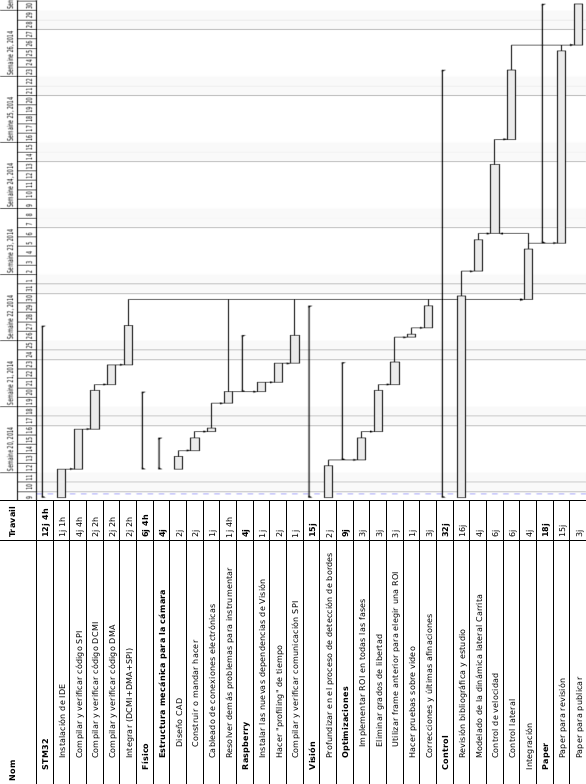
\includegraphics[height=1.3\textwidth]{fig/ganttscaled}\\
\caption{Gantt chart for the first two months.}
\label{fig_ganttA}
\end{center}
\end{figure}

\subsection{Camera mount mechanism drawings}
\begin{figure}[ht!]
\begin{center}
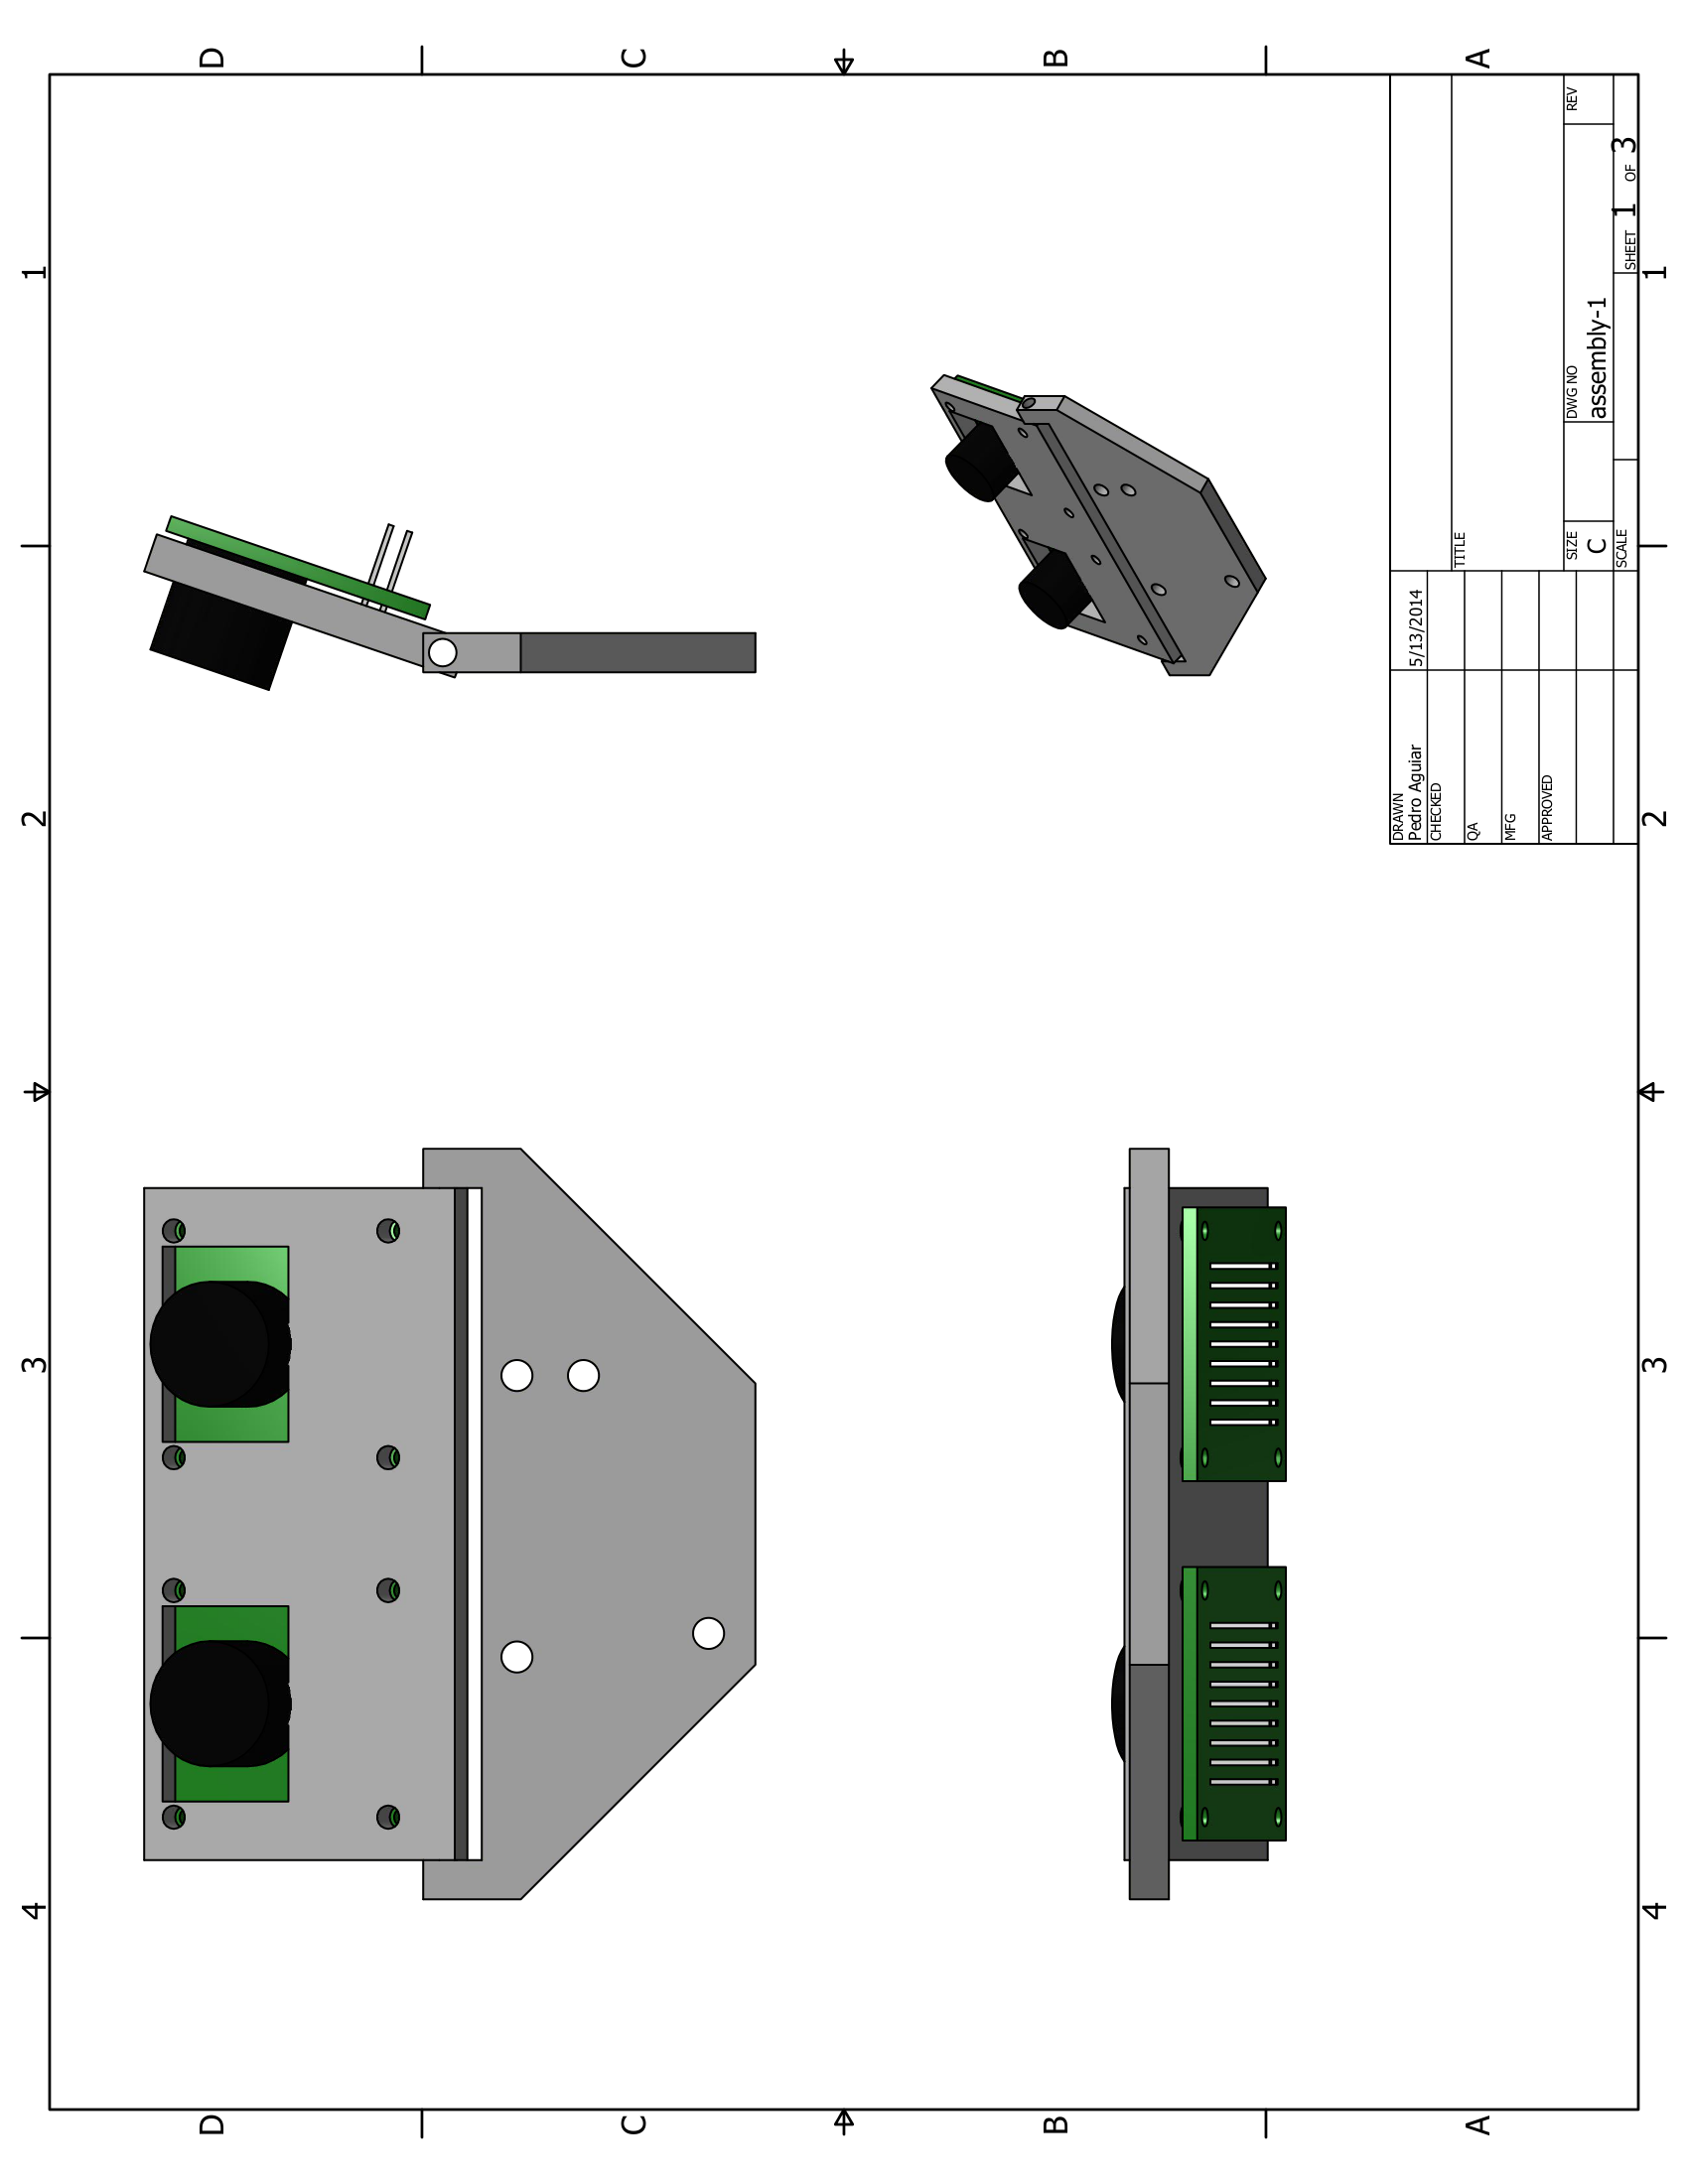
\includegraphics[height=1.2\textwidth]{fig/cammountp1}\\
\caption{Camera mount mechanism drawings: Assembled camera mount.}
\label{fig_cammountp1}
\end{center}
\end{figure}

\begin{figure}[ht!]
\begin{center}
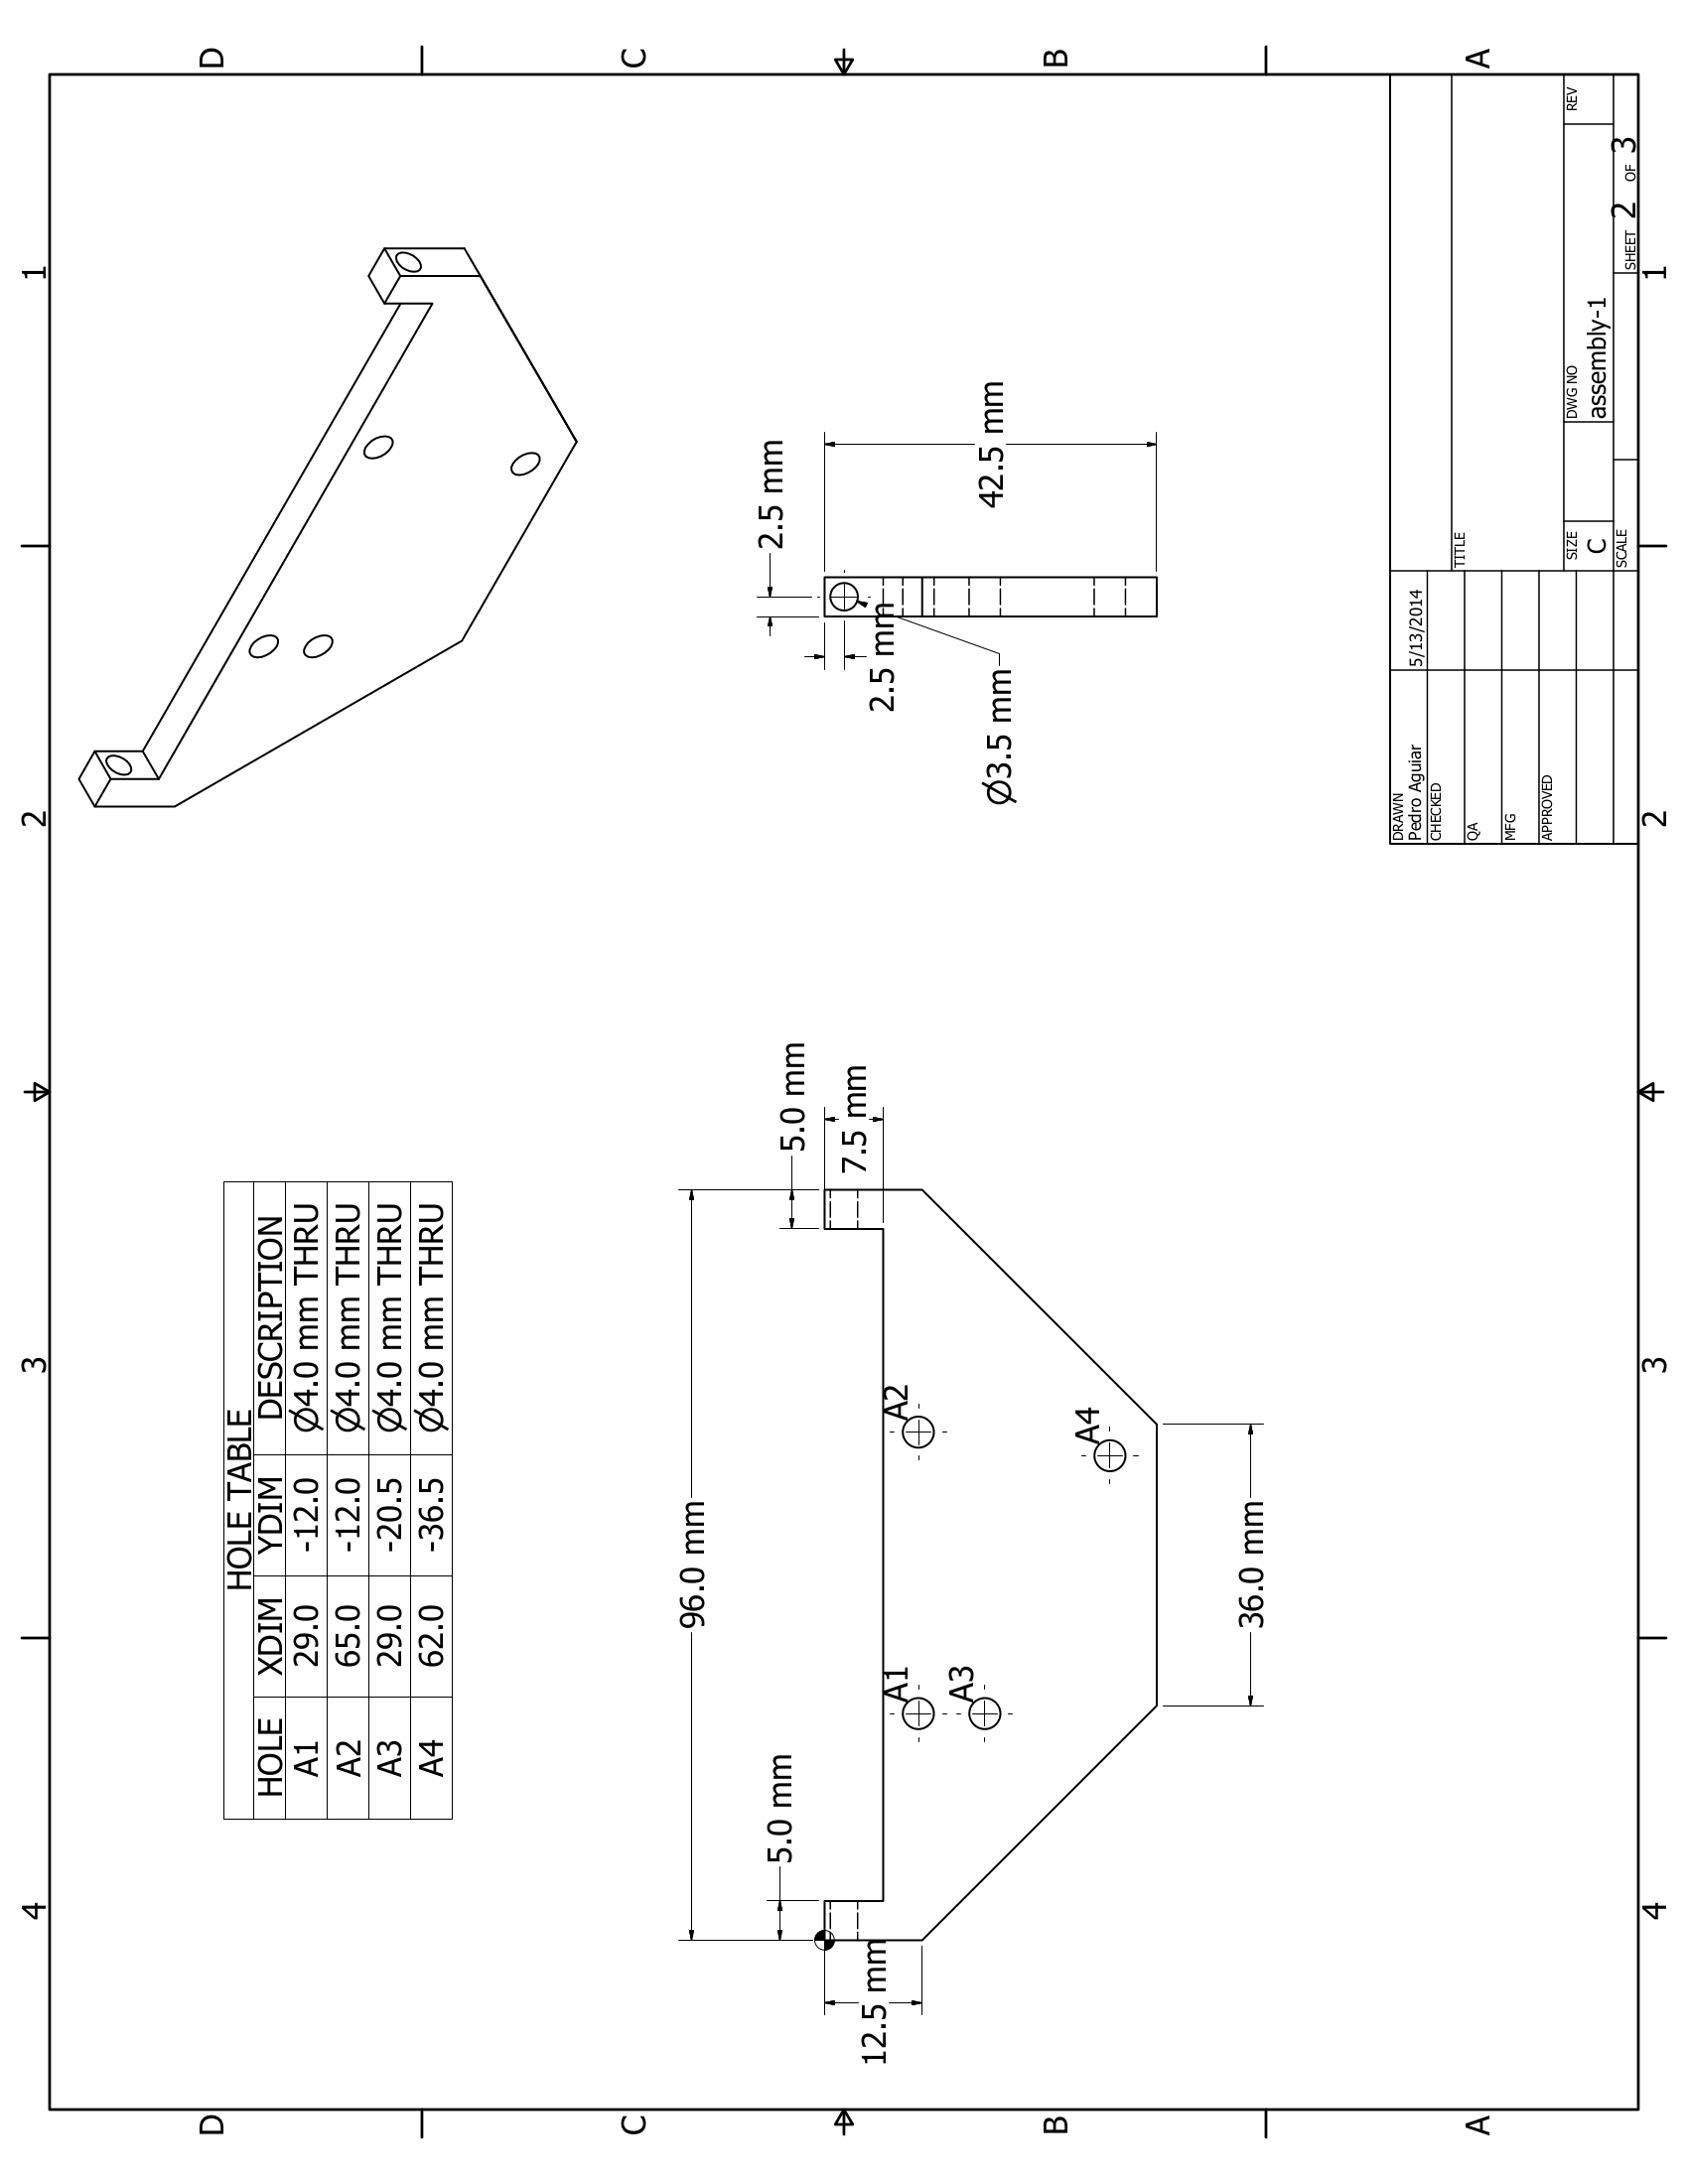
\includegraphics[height=1.2\textwidth]{fig/cammountp2}\\
\caption{Camera mount mechanism drawings: camera part.}
\label{fig_cammountp2}
\end{center}
\end{figure}

\begin{figure}[ht!]
\begin{center}
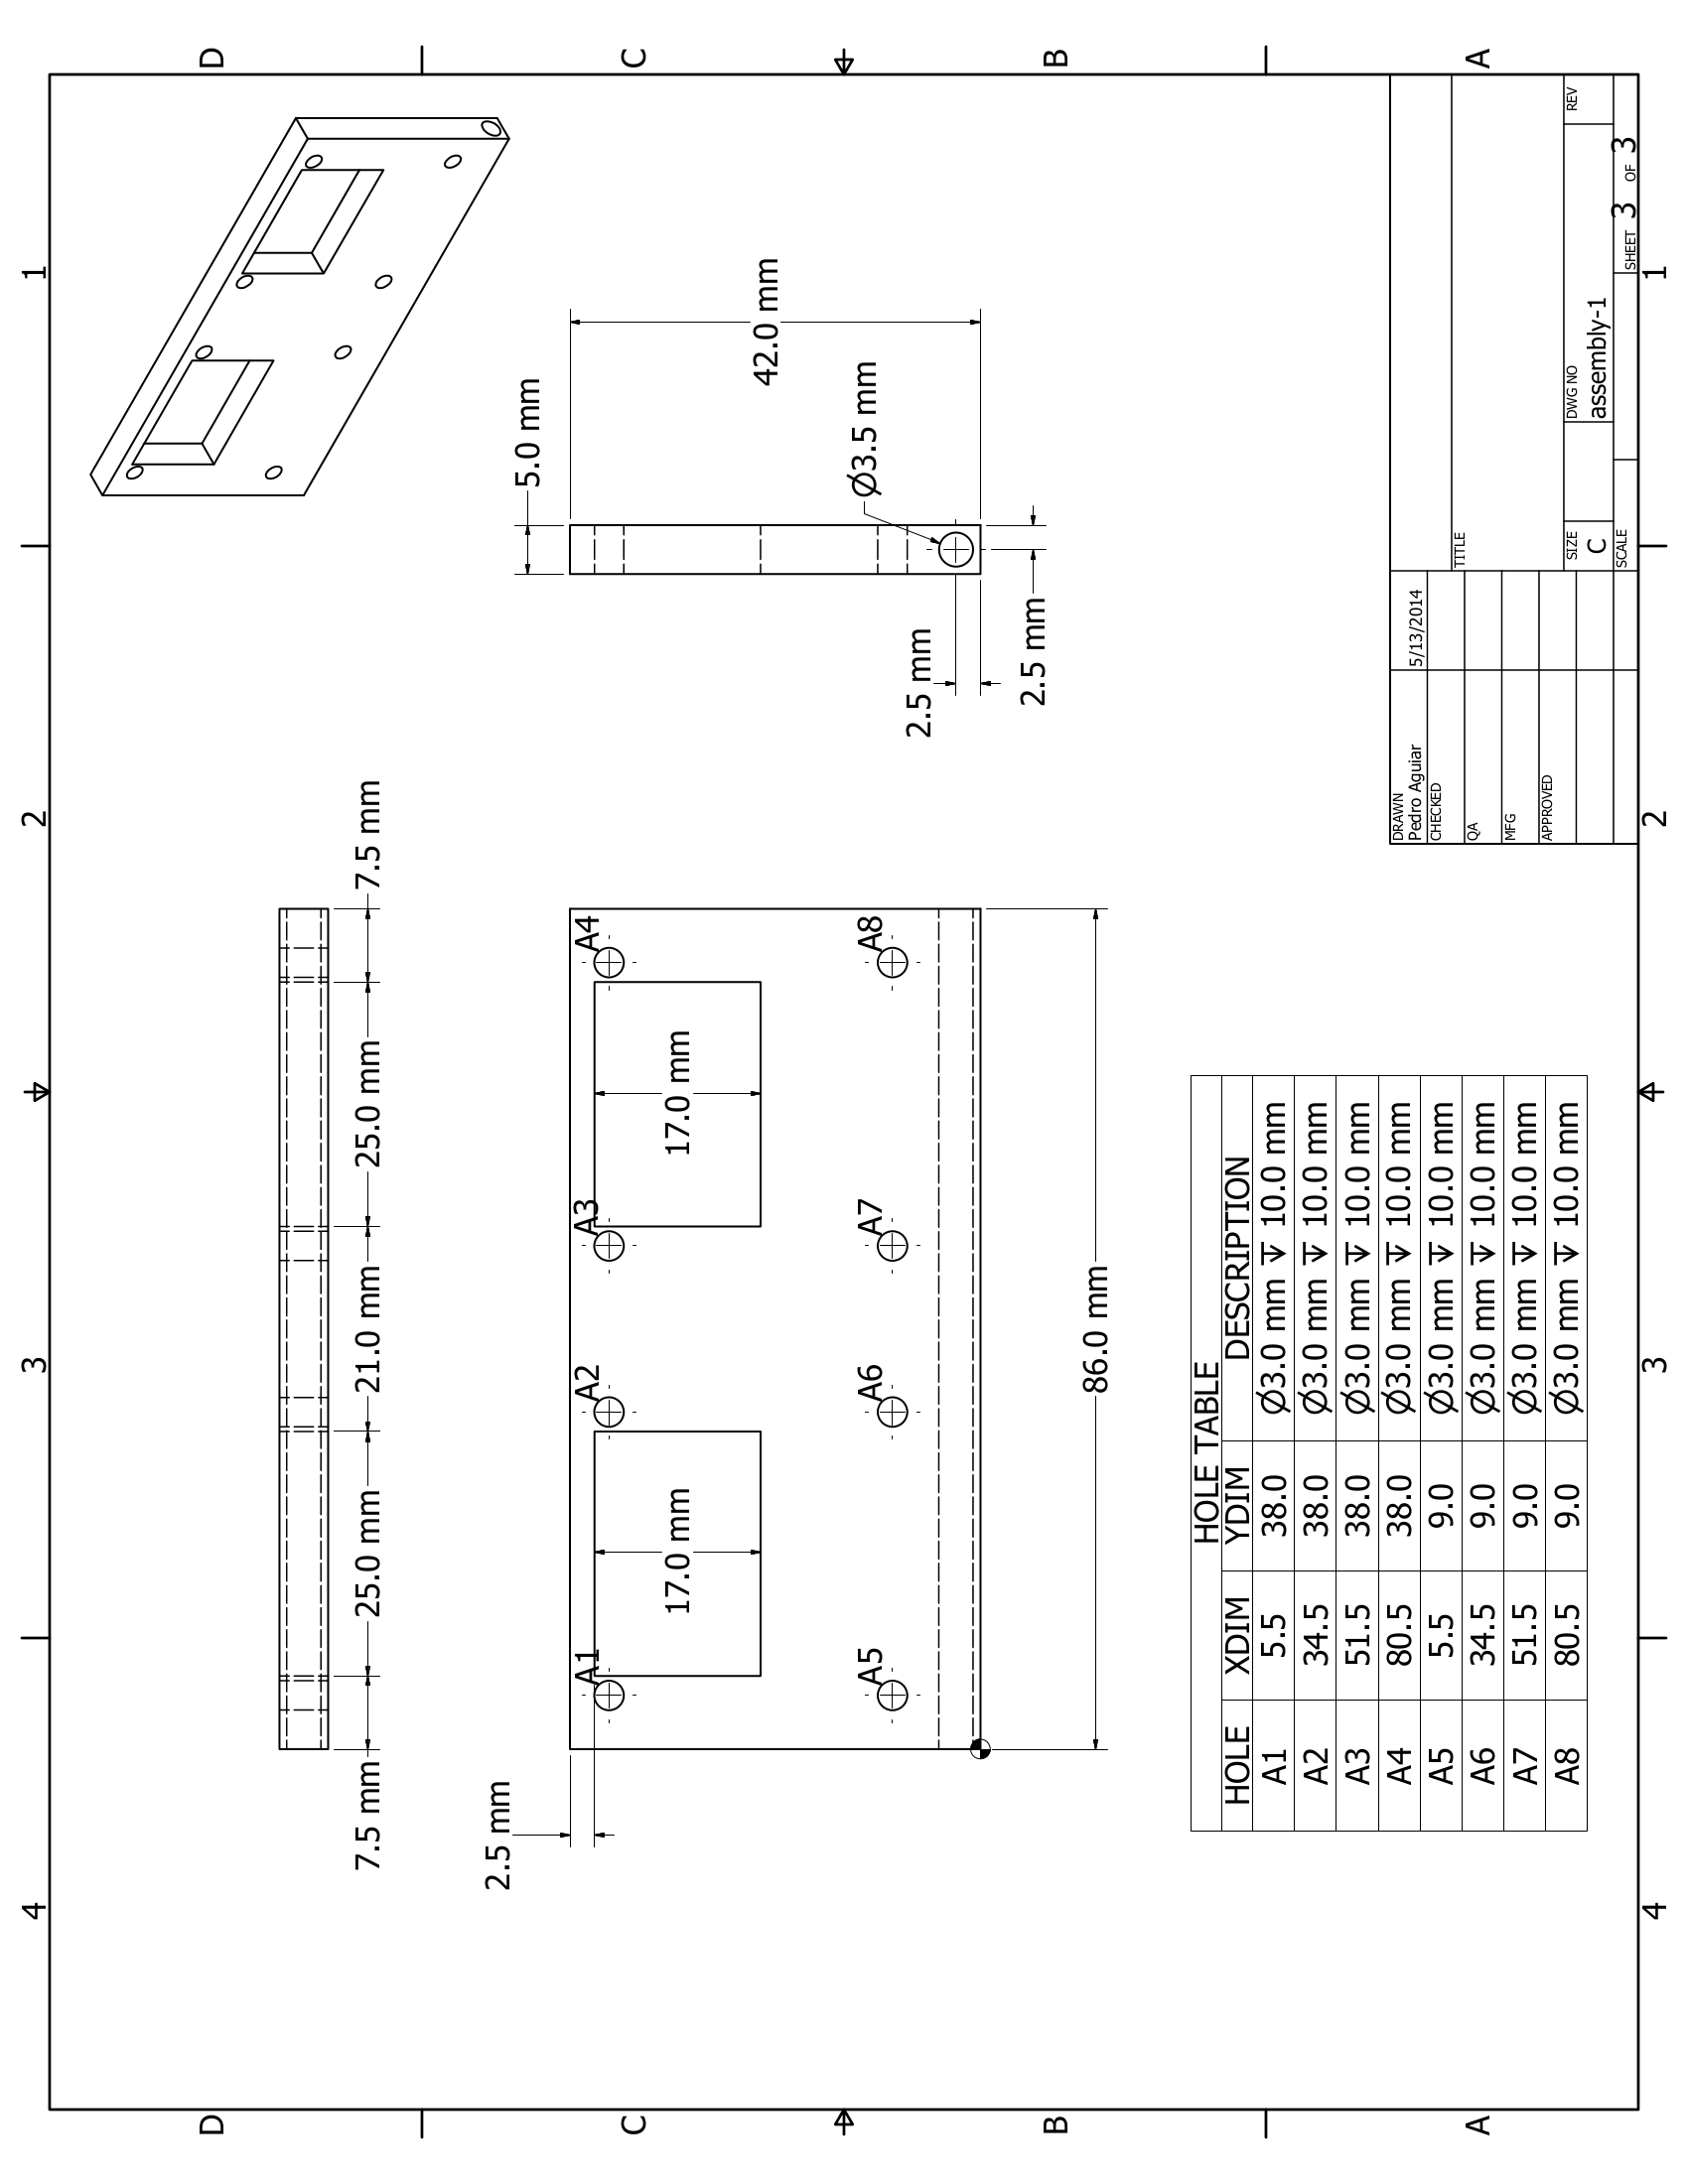
\includegraphics[height=1.2\textwidth]{fig/cammountp3}\\
\caption{Camera mount mechanism drawings: Carrita's part.}
\label{fig_cammountp3}
\end{center}
\end{figure}

\clearpage

\begin{thebibliography}{9}
 \bibitem{cummings}
	Chris Cummings,
	\emph{Gpu accelerated image processing on raspberry pi}. http://youtu.be/yQZISXIFjaQ

 \bibitem{dubska}
	Markéta Dubská, Adam Herout,
	\emph{Real-Time Detection of Lines using Parallel Coordinates and OpenGL}. 

\end{thebibliography}

\end{document}
